\subsection{Class Diagrams}


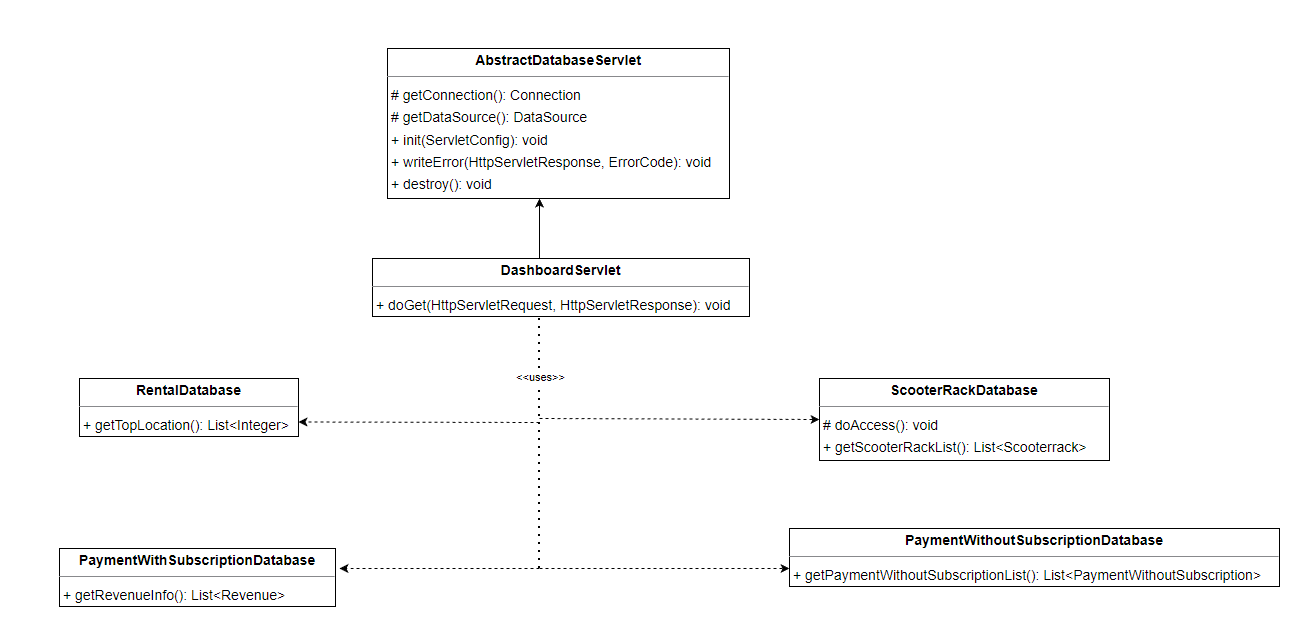
\includegraphics[scale=0.5]{sections/DLL/dashboard-servlet_CD.png}
This class diagram represents the classes involved in the dashboard servlet, which manages the dashboard page.
This servlet uses the classes shown to access the database.


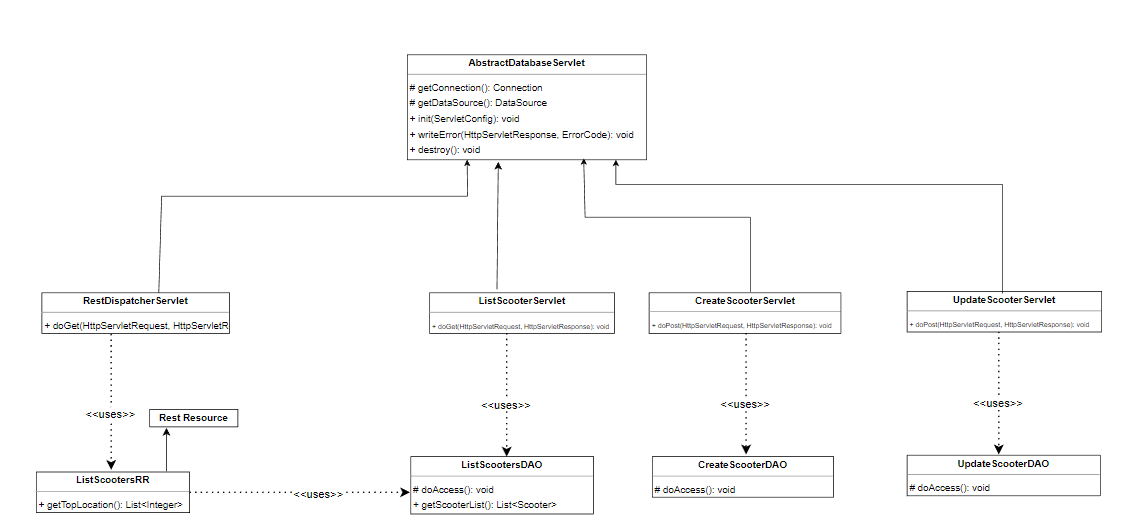
\includegraphics[scale=0.5]{sections/DLL/scooter-servlet-rest_CD.png}

This second class diagram represents one of the manage pages servlets and rest.
The manage pages are model, scooter, scooterrack, rental, payment methods, customer and subscription.
On this pages we can interact with the respective tables of the database, for example viewing the list, adding or editing that entity.
In this case we shown the scooter entity, we have a servlet for viewing the list of scooters, one for adding a new scooter and one for editing an already existant scooter.
Then we also provide the REST API for getting the list of scooters.
Both the rest and the servlets use some classes to access the database, shown in the diagram.